%%%%%%%%%%%%%%%%%%%%%%%%%%%%%%%%%%%%%%%%%%%%%%%%%
%%%%%%%%%%%%%%%%%%%%%%%%%%%%%%%%%%%%%%%%%%%%%%%%%

\chapter{Foraging}
\label{chap:second}

%%%%%%%%%%%%%%%%%%%%%%%%%%%%%%%%%%%%%%%%%%%%%%%%%
%%%%%%%%%%%%%%%%%%%%%%%%%%%%%%%%%%%%%%%%%%%%%%%%%

In swarm robotics, robot foraging has become a benchmark problem due to its complex nature involving the coordination of numerous sub-tasks and is also one of the swarm robotics problems that has some very obvious useful applications. This chapter aims to provide an in-depth review of what foraging is, how different social insects forage as well as provide a review of existing foraging algorithms in swarm robotics. The definition of foraging in swarm robotics is discussed in Section~\ref{sec:second:definition}, while Section~\ref{foraging:biologicalinspiration} discusses the biological techniques for foraging in social insects - ants and bees. Section~\ref{sec:second:types} addresses a taxonomy of the types of swarm robotic foraging algorithms and the challenges that foraging algorithms must address are discussed in Section~\ref{challengesinforaging}. Existing swarm robotics foraging algorithms are outlined in Section~\ref{sec:second:existingsolution} and prioritized foraging is defined and discussed in Section~
\ref{sec:second:prioritizedforaging}. Lastly, the chapter is summarized in Section~\ref{foraging:summary}. 


%%%%%%%%%%%%%%%%%%%%%%%%%%%%%%%%%%%%%%%%%%%%%%%%%
%%%%%%%%%%%%%%%%%%%%%%%%%%%%%%%%%%%%%%%%%%%%%%%%%

\section{Definition}
\label{sec:second:definition}

Foraging was initially addressed by biologists, particularly in the foraging behaviour of ants \cite{holldobler1990ants,bernstein1974seasonal}, bees \cite{seeley2009wisdom} and bacteria \cite{resnick1994turtles}. Foraging has a variety of real-life applications such as search and rescue \cite{jennings1997cooperative,murphy2000biomimetic}, and waste clean-up \cite{balch1995io}. Numerous swarm robotics algorithms have been developed to improve robustness, time and energy efficiency of the foraging process for multiple variations of the foraging problem as outlined in \cite{winfield2009foraging}. 

Foraging is the act of searching for and collection (or capturing) food for storage and consumption \cite{winfield2009foraging}. Foraging is an important problem that was first addressed by biologists in the examination of nature, particularly with the foraging behaviour of ants and bacteria. In a robot context, foraging is defined as the search and collection of scattered objects in an environment and returning those objects to a collection point.

The foraging sub-tasks involve the efficient search and collection of food, homing whilst carrying food to the nest site and then deposition of the food item in the nest before returning to foraging. Effective foraging requires co-operation using signals or direct cooperation of individuals in order to transport food items too large for individual transport. The foraging process has been adapted for numerous foraging problems and for different types of robots and is often replaced completely with more complex models, including communication components and division of labour. 
%TODO: Add citations. 

\section{Biological Inspiration}
\label{foraging:biologicalinspiration}
As with many swarm robotics problems, the inspiration comes from nature - in particular, social insects such as Ants and Honeybees. This section describes the biological models that are used in the algorithms derived by this thesis. 

\label{sec:second:biological}

\subsection{Ants}
%Ants
The study of ants has revealed that impressive emergent activities can be achieved with  simple agents with only a few simple rules. Ants use a form of communication known as stigmergy \cite{dorigo2000ant}. Stigmergy is where ants deposit a substance known as pheromone on the paths between the nest and the food source. Other ants can detect this pheromone and will tend to follow paths which have greater amount of pheromone deposits. Ant stigmergy has been modelled in numerous swarm intelligence techniques such as ant colony optimization and ant systems \cite{dorigo2006ant, dorigo2010ant}. 
 
Although algorithms based on ant foraging behaviour are used to solve optimization problems, the algorithms are often difficult to replicate in a real-life robotic environment since most of the techniques need to model stigmergy. A robotics algorithm that uses pheromone requires robots to be equipped with a substance-distributor, beacon-deployer or complex communication that simulates pheromone \cite{hoff2010two}.

%TODO: Mention each other the pheromone using robotic techniques - a review so to say. 

The desert ant (\textit{Cataglyphis bicolor}) does not make use of stigmergy to forage, as pheromone deposited on desert sand would be blown away by the wind. Instead, desert ants use a technique called path integration for navigation to relocate food sources that have already been found by random exploration \cite{collett1998local,wehner2003desert} as illustrated by Fig. \ref{pathintegration}. An overall heading and distance from the nest is maintained as the desert ant explores. As a result, a shortcut back to the nest is calculated in order to minimize heat stress. A human would solve this problem using vector addition, however ants have been shown to use a simpler approximation, which performs adequately, despite the addition of noise \cite{muller1988path}. Path integration (PI), more commonly known as dead reckoning, is a key evolutionary aspect gained from living in the hot barren desert. When path integration fails, the ant resorts to using landmarks, such as the sun, for navigation \cite{collett1998local}. 

\begin{figure} [h]
	\centering
	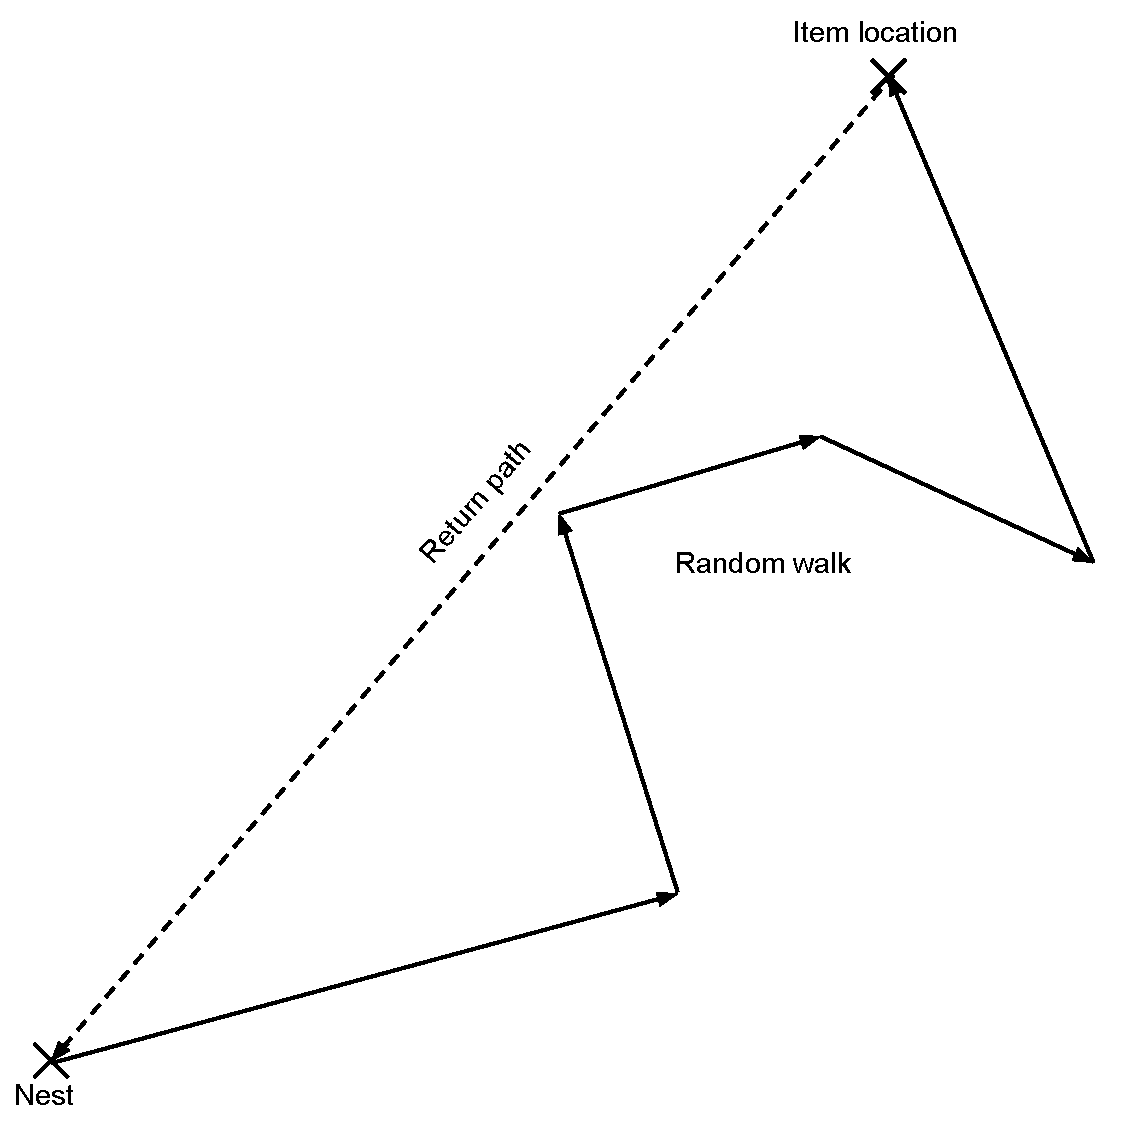
\includegraphics[width=0.65\textwidth]{chapters/chapter2/figures/PathIntegration.pdf}
	\caption{Path Integration }
	\label{pathintegration}
\end{figure}

Due to the lack of pheromone, the desert ant is thus simpler to model for real-robot interaction. Desert ant foraging has been modelled in \cite{moller1998modeling,hecker2012formica,}. Hecker et al \cite{hecker2012formica} performed experiments using a small set of robots in a small arena on different environment types where two algorithms were evaluated: one based on the desert ant foraging and one including pheromone-like communication. It was shown that communication improved performance; however, the desert-ant algorithm still performed comparatively well. 

\subsection{Honey bee}

Bees have an impressive set of abilities considering the simplicity a single individual. They have the ability to remember colour and shape of flowers \cite{zhang2006honeybee} and in terms of navigation, they are able to learn local features and routes due to well-developed learning and memorizing capacities \cite{menzel2001cognitive}. Honey-bees are even time aware \cite{moore1989influence}. 

Similarly to ants, honey bees have efficient division of labour between different functions in the hive such as foraging and brood-care. Within foraging itself, honey bees perform division of labour specific to the foraging roles. Honey bee foraging is made up of three different roles \cite{seeley2009wisdom} namely employed foraging, unemployed foraging and scouting. Scouts explore the environment to locate new food sources. Once a source has been found, scouts return to the hive to communicate information about the located food source. To communicate the foraging information, scout bees perform a waggle-dance on the hive, containing information about the distance and bearing of the resource. The communication of a good foraging site is known as recruitment. 

Unemployed foragers wait on the dance floor, evaluating the dances of the scout bees. An unemployed bee chooses a location described by the scout bees, and becomes an employed forager. Employed forager bees use the information about the resource, attempt to locate the source, load themselves with food and return to the hive where unemployed foragers are ready to offload the food. Jansen \cite{janson2007searching} suggests that unemployed bees become exploring scouts when they do not detect any dancing scout bees. 

\subsection{Other}
\label{otherforaginginspirations}
%Not sure where to put this but I think it deserves a mention
Foraging is modelled in the swarm intelligence field. Besides ants and bees, other creatures are also looked to for inspiration.

The foraging behaviour of $E. coli$ bacteria is used for inspiration for a computational intelligence algorithm \cite{passino2010bacterial} and particle swarm optimization is, for instance based on the flocking behaviour of birds - a flocking behaviour exhibited when finding food, amongst other things \cite{kennedy1995particle}. 

The predator prey models could also be considered a foraging task with items with changing position. These models are often used with other swarm intelligence techniques, for use in multi-objective optimization problems \cite{nolfi1998coevolving}.


\section{Types of Robot Foraging}
\label{sec:second:types}

Foraging is a popular problem due to the vast opportunity for application. The foraging problem has been adapted into many different variations. Thus it is beneficial to present a taxonomy of robot foraging that can used to classify existing research about foraging as well as contextualize the specific foraging problems addressed by this thesis. Multiple taxonomies have been developed as robot foraging research has progressed \cite{oster1978caste,ostergaard2001emergent}, however a more recent taxonomy is presented in \cite{winfield2009foraging} which presents and discusses a much more complete foraging taxonomy. The taxonomy classifies foraging solutions based on characteristics of four major axes: the foraging environment, robots used for foraging, performance aspects and the foraging strategy used. Each of these major axes have a number of minor categories which are outlined in the table below.  

The environment classification axis includes addressing aspects such as search space itself, the type and placements of objects as well as the quantity of sinks. The robot aspect refers to qualities such as  the quantity of robots along with the robot's sensory, power and actuation capabilities. The performance axis characterises robot foraging on the the goal of the research such as energy gained or time taken to forage. The strategy axis characterizes algorithms by how the algorithm goes about solving the foraging problem. 

\begin{table}
\centering
    \caption{Winfield's Robot Foraging Taxonomy}
    \label{foragingtaxonomytable_part1}
    
\begin{tabular}{ | c | c | c |}
	\hline
	Major Axis & Minor Axis & Value  \\ \hline
	\multirow{13}{*}{Environment}
		& \multirow{2}{*}{Search space} 
			& Unbounded \\  
		& 	& Constrained \\ \cline{2-3}
		& \multirow{3}{*}{Source Areas} 
			& Single limited \\ 
		&	& Single unlimited \\
		&	& Multiple \\ \cline{2-3}
		& \multirow{2}{*}{Sinks} 
			& Single \\
		&	& Multiple \\ \cline{2-3}
		& \multirow{3}{*}{Object types} 
			& Single static \\
		&	& Multiple static \\
		&	& Single active \\ \cline{2-3}
		& \multirow{3}{*}{Object placement} 
			& Fixed known locations \\
		&	& Uniform Distributions \\
		&	& Clustered \\\hline
	\multirow{16}{*}{Robot(s)}
		& \multirow{2}{*}{Number} 
			& Single \\  
		& 	& Multiple \\ \cline{2-3}
		& \multirow{3}{*}{Type} 
			& Homogenous \\ 
		&	& Heterogenous \\ \cline{2-3}
		& \multirow{2}{*}{Object Sensing} 
			& Limited range \\
		&	& Unlimited range\\ \cline{2-3}
		& \multirow{3}{*}{Localization} 
			& None \\
		&	& Relative \\
		&	& Absolute \\ \cline{2-3}
		& \multirow{3}{*}{Communications} 
			& None \\
		&	& Near \\
		&	& Infinite \\\cline{2-3}
		& \multirow{3}{*}{Power} 
			& Limited \\
		&	& Forage \\
		&	& Unlimited \\\hline
\end{tabular}
\end{table}

\begin{table}
\centering
    \caption{Winfield's Robot Foraging Taxonomy Part 2}
    \label{foragingtaxonomytable_part2}
    
\begin{tabular}{ | c | c | c |}
\hline
	Major Axis & Minor Axis & Value  \\ \hline
	\multirow{6}{*}{Performance}
		& \multirow{3}{*}{Time} 
			& Fixed \\  
		& 	& Minimum \\ 
		& 	& Unlimited \\ \cline{2-3}
		& \multirow{3}{*}{Energy} 
			& Fixed \\ 
		& 	& Minimum \\ 
		&	& Unlimited \\ \hline
	\multirow{6}{*}{Strategy}	
		& \multirow{5}{*}{Search} 
			& Limited range \\
		&	& Geometrical pattern\\
		&	& Trail following\\
		&	& Follow other robots\\
		&	& In teams\\ \cline{2-3}
		& \multirow{2}{*}{Grabbing} 
			& Single \\
		&	& Cooperative \\ \cline{2-3}
		& \multirow{2}{*}{Transport} 
			& Single \\
		&	& Cooperative \\ \cline{2-3}
		& \multirow{3}{*}{Homing} 
			& Self navigation \\
		&	& Home on beacon \\
		&	& Follow trail \\\cline{2-3}
		& \multirow{3}{*}{Recruitment} 
			& None \\
		&	& Direct \\
		&	& Indirect \\\cline{2-3}
		& \multirow{3}{*}{Coordination} 
			& None \\
		&	& Self-organized \\
		&	&  Central control \\
		&	& Master slave \\\hline
\end{tabular}
\end{table}
%TODO: Add caption to table if we use it. 

%%%%%%%%%%%%%%%%%%%%%%%%%%%%%%%%%%%%%%%%%%%%%%%%%

\section{Challenges in Foraging}
\label{challengesinforaging}
%TODO: Expand on challenges in foraging. 
Foraging for humans is a near trivial problem. Most children can walk around and retrieve blocks and return them to a single source. The seemingly simple sub-activities required by foraging such as identification and grasping are often relatively complex for robots to perform. Some of the areas which are problematic for robots in a foraging concept are presented as follows:

\begin{itemize}
\item Physical - Despite how far robotics has come as a field, there are still tasks that are trivial for humans, but still very complex for most robots. For instance, challenge of picking up items and moving them to another location requires a fair amount of research, decent quality sensors and time-consuming amount of calibration. 

\item Environmental - Although research can be performed in a controlled environment, for foraging to truly occur in real-life, environmental factors have to be taken into consideration. Environmental factors such as light, moisture, quality of the surface the robots forage on, often make a robotic solution a complex, non-viable, non-robust or expensive operation. 

\item Search with local sensors - Since global sensors such as GPS location can't always be used in all environments, the problem of how to find items with or without a global view of the environment and how to effectively guide the search optimally becomes a large issue. Swarms need to learn techniques of exploiting local information about the environment and use local communication in order to maintain environmental knowledge to aid search. 

\item Localization - Localization is the ability for a robot can depict their position in the environment. Without a global knowledge, similarly to search, the problem of a robot knowing where it is in relation to the boundaries of the environment or other known locations and robots also becomes difficult.

\item Energy - One of the predominant problems in much modern technology is energy conservation. As technology gets smaller, battery technology also has to become smaller but the devices still must should maintain charge for long periods. As robots get smaller, batteries are also getting smaller so energy conservation and automatic charging become an important problem in swarm robotics that needs to be solved.

\end{itemize}

Due to the complexity of the foraging problem, existing research will often simplify parts of the problem in order to focus on certain aspects. Simplification is often through use of simulators or assuming certain environments or technological capabilities of the robots. 

\section{Foraging Algorithms}
\label{sec:second:existingsolution}


This section discusses some foraging solutions that have been developed as well as looks at the different types of foraging problems. 

%Mention the current attempts at foraging. 
%Keep in mind to mention the papers about the techniques that I am comparing. 
%The desert ant, bee techniques, basic ones. 
%Mention but don't go into details about papers that attempt very specific ones.
%Insect Inspired
%----------------------------
Insects swarms are used as inspiration throughout swarm robotics due to their robust and flexible nature. Ants utilize pheromones which is a robust strategy for local interactions and would prove useful in hazardous environments. Section \ref{sec:second:natureinspired} discusses nature-inspired foraging algorithms 
%citation & write better.
 
\subsection{Nature-inspired Swarm Robotics Foraging Algorithms}
\label{sec:second:natureinspired}

%TODO: Add introduction to section
%TODO: Review

\subsubsection{Ant-inspired Foraging Algorithms}

%Blazing a trail => Nice paper - need to discuss more. Maybe in navigation
Vaughan presents a swarm robotic algorithm allowing for robust transportation of items from a single source to a single sink in an environment with spatial constraints \cite{vaughan2000blazing}. The algorithm presented makes use of both ant-like and bee-like foraging techniques. The ants broadcast the landmarks in the area for odometric localization as well as uses a form of the  honey bee "waggle dance" that communicates the direction of the food source from the robot that has found the food source to other robots. The robots use a technique called path integration utilized by both ants and bees in order to maintain position and heading estimate. Using these techniques the robots communicate multi-segment paths. These communications occur globally. This technique suffers from accumulation of localization errors over time due to the use of global communication. Local communication is preferred for the algorithms developed in this study.   %Our robot algorithms can reaign the sink %citations required!!!! %necessary? Worth a mention. 


%ANTS%
Hoff \cite{hoff2010two} classifies different types of ant-inspired pheromone-based foraging algorithms by how the pheromones are represented: physical marks \cite{alcoholfromants2012}, use of existing communication channels such as sharing over wireless networks as well as virtual pheromone. %Read further

%DoL in a Group of Robots Inspired by Ants Foraging Behaviour - Labella + Dorigo
Labella et al \cite{labella2006division} propose a foraging model inspired by the foraging of ants, where individual robots adapt to the environment using only locally available information. The adaption allows for effective division of labour to occur. The probability $p1$ that a robot will changed from rest to searching is adapted upon return to the sink and from deposit to rest. If a robot fails to forage any prey after searching for a specified maximum time, then the robot returns and rests. 
The adaption rule increases or decreases $p1$ by a constant $\Delta$ that is multiplied by the number of consecutive successes or failures. The study showed that adaption improved the amount of time spent not at rest. The advantage to this type of algorithm is its simplicity as no communication is required to regulate the number of robots. As pointed out, there is a global negative effect on overall efficiency at large group sizes. This is to be expected, but is not a serious problem since less energy is used, and this would be an advantage when energy is a scarce resource. %rephrase%
%Different from the problem proposed in this study as different priorities of items are not considered
%Come back and do a bit later. 
%Says prey

\begin{figure}
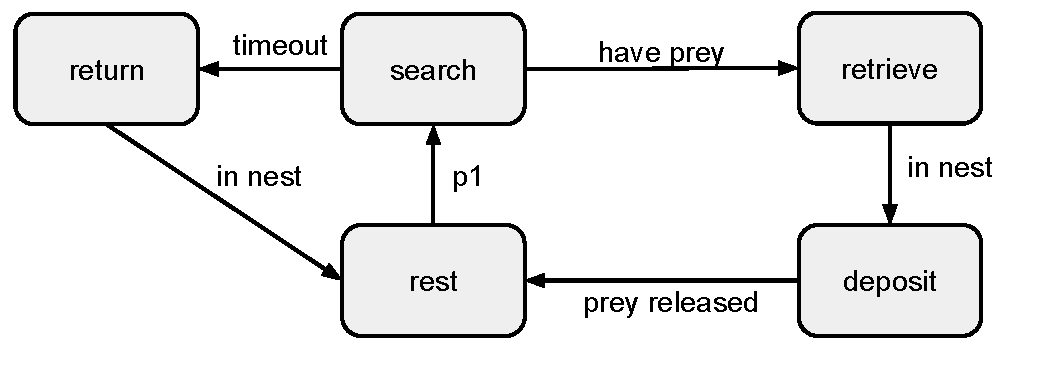
\includegraphics[width=\textwidth]{chapters/chapter2/figures/LabellaFSM.pdf}
\caption{Simplified finite state machine for Labella division of labour algorithm. }
\end{figure} 

Hoff \cite{hoff2010two} proposes a two ant-based foraging algorithm which do not require marking the physical environment. Instead, robots themselves become pheromone markers. The algorithms differ in the manner in which the beacon-to-pheromone role is chosen. 

Virtual pheromone algorithm functions as follows: Two pheromone trails are created - one trail from the source to the food and another trail from the source to the nest. The trail is created by robots: During execution, robots stop exploration and become pheromone beacons. The pheromone beacon robots simply broadcast a floating point number known as virtual pheromone. 
Local direct communications are used to transmit the virtual pheromone value.

The second technique uses cardinality where if a robot can hear 2 or more beacons then the robot stays a walker else the robot becomes a beacon. 
%Etc etc add more from paper!!!!

The advantage of using this technique over the other mentioned pheromone techniques is that robots are simpler due to simpler communication mechanisms as well as the lack of need for complex beacon deployment systems. Experiments are conducted with and without obstacles and a real-world simulator is used. The result show that congestion effects performance the most at high robot density. %write more in more detail. The cardin

\subsubsection{Bee-inspired Foraging Algorithms}
Bee swarms have been used in swarm robotics for problems such as path planning \cite{lin2009chaotic}, aggregation \cite{kernbach2009re}, collective perception \cite{schmickl2007collective}.%Relevant? Not sure. 

%TODO: Explain each example application
Foraging algorithms have been developed that simulate a simplified honey bee recruitment in \cite{alers2014biologically}, which focuses on an actual robot demonstration of the technique using a turtle robot. Prior work focuses on implementing the same algorithm on e-pucks. The algorithm consists of two phases: an exploratory phase followed by an exploitive phase. Initially, all robots are located around the hive. In the exploratory phase, all robots perform a random search with a levy distribution until a food source is found by a robot. The exploitation phase begins where the robot that located the food returns to the hive and communicates the location to other members of the robot swarm. The other robots are recruited and begin to commute between the hive and the food source, transporting virtual food. This algorithm claims to exhibit three behaviours of bees: waiting around the hive, exploring the environment and foraging. Unlike bees, the algorithm used does not consider the division of labour between foragers, explorers and waiting robots, but rather uses an extremely simple model for bees which can only exploit a single food source. The robots use path integration in order to remember the location of the food source, and use a north-star type navigation in order to locate the hive. The path integration vector gets communicated to the other robots which use the vector to guide them to the food source. 

%\subsubsection{Other Nature-inspired Foraging Algorithms}
%TODO: Research and add 

%\subsection{Other Algorithms}
%\label{sec:second:otheralgorithms}
%TODO: Introduction to subsection

\subsection{Standard foraging}


%Fotan & Mataric
Schneider \cite{schneider1998territorial}, in order to reduce the interference caused by collisions, develop an algorithm to split the foraging environment into bounded areas for which a robot is in charge of. The sink area of one robot is the source area for the next, resulting in the emergence of bucket brigading behaviour. The bucket brigading algorithm is not suitable to environments where the size of the environment is not known - unless an algorithm is developed that will effectively allow a swarm of robots to divide the area. The algorithm is thus not suitable for comparison for the current study. The failure of a robot induces readjustment of territories in order to effectively cover the foraging area. Global information about the environment is used and as a result the algorithm is not suitable for comparison. %Reread to figure out if initial distribution algorithm exists

%Mataric
\O stergaard \cite{ostergaard2001emergent} determines that there is a finite number of any particular type of robot that is optimal for performing a foraging task. Mataric compares the algorithm to a naive algorithm which represents the baseline foraging task with no improvements. The naive algorithm in the thesis as a baseline comparison measure and is discussed in more detail in further chapters. Mataric found that if too many robots were allocated to the environment then extreme amounts of interference occurred which decreased the performance of the algorithm. Emergent bucket brigading was shown to perform better than naive in highly constrained environments however naive performed better in open environments. Algorithms are tested in environments of differing difficulties. %Need to read this paper to check which one these details came from. Also DO the thing for his name


%Goldberg + Mataric
Goldberg and Mataric \cite{Goldberg01designand} address the foraging problem with multiple sources and sink areas in an open field environment. The study focuses on interference reduction by making use of a dominance hierarchy - only the dominant robot near the sink can take an item to the sink. %mentioned PACK foraging. read up

%Mataric and Werger
Mataric \cite{werger1996robotic} and Werner discuss produced an algorithm where chains of robots are formed and the robots forage in circular excursions. The length of the change is then adusted according to the amount of food found by the foragers. %No idea how this works - read up. 
 
%Swarming Robots: Foraging Behaviour of Simple Multi-Robot System
Sugawara \cite{sugawara2002swarming} implements a foraging solution for a single food source. The algorithm is based on naive foraging however utilizes simple communication. A robot will stay and broadcast a light signal on finding an item. Other robots are attacted to the light signal based on an angular velocity equation. This differs from the techniques used in this thesis as all food sources communicated with equal weight where as the quality of a food source is evaluated by the honey bee algorithm.

%Alexandre Campo 2006 - Efficient multi-foraging robotics
\subsection{Multi-foraging}
Multi-foraging is defined as a type of foraging problem where instead  multiple object types are required to be foraged. \cite{Balch99rewardand}. The types of objects can have different characteristics and can be collected together or separately.

%Adaptive DoL in Large-scale Minimalist MultiRobot systems - Mataric.
%2 types of items 
Jones et al \cite{jones2003adaptive} describe a version of the problem where there exist two types of items and items are consumed instead of transported to the sink and as items are consumed, the same type of item is placed at a random spot in the arena. Robots signal what type of item they are foraging by a coloured light which other robots use to build a local history of the number of robots they have seen that are allocated to each item type. A history of the number of observed items of each type is also collected. The division of labour capability is formed by estimating the current division of labour of the group by  using the described local observations. The estimations are then used to determine the probability of changing from foraging the current item type to the other type. 

%\begin{equation}
% P(Green - Red) = \left\ {
%	\begin{array} {l l}
%		(GR - GP_*(1-GP) & \quad \textrm{if GR \geq GP} \\
%		0, & \quad \textrm{otherwise}
%	\end{array}
% \right.
%\end{equation} 

%		(RR- RP)*(1-RP) & \quad \text{if RR $\geq RP$
%%%%DoL$
Campo \cite{campo2007efficient} performs a study in order to identify characteristics of efficient multi-foraging behaviour.  A mathematical model is developed and validated to predict optimal foraging behaviour and thus allows absolute evaluation of the proposed decision algorithm. The proposed foraging decision algorithm utilizes the amount of other robots encountered as well as the amount of prey encountered to only allocate enough robots foraging  so that remaining robots can spare energy. A measure is proposed that estimates the instantaneous energy that a robot group can gain, which each robot uses to guide the search process. 
%Need to add discussion
%Says prey

Balch \cite{balch1999impact} develops a technique for multi-foraging and determining the impact of robot diversity on multi-foraging performance. This thesis's does not consider robot diversity since robots are homogenous.

%%%%%%%%%%%%%%%%%%%%%%%%%%%%%%%%%%%%%%%%%%%%%%%%%
%%%%%%%%%%%%%%%%%%%%%%%%%%%%%%%%%%%%%%%%%%%%%%%%%


\section{Prioritized Foraging}
\label{sec:second:prioritizedforaging}

%Focus on the robots used, the model used and the experiments performed

The multi-foraging problem is a more complex version of standard foraging, where more than one type of item must be foraged to a separate sink \cite{balch1999impact}. That in mind, the prioritized foraging problem, shown in Fig.\ref{prioritizedforaging}, is defined as a modified version of the multi-foraging problem where an environment has two types of items: prioritized items and non-prioritized items. The goal is to forage all the items of the prioritized type. The possibility exists that prioritized items become trapped among non-prioritized items and thus the non-prioritized items need to be removed from the environment to clear an access route to the prioritized items. 

The prioritized foraging problem has increased difficulty due the fact that  foraging the non-prioritized item more than required will result in a waste of time and energy. The goal of research in prioritized foraging is to develop an algorithm to efficiently adapt the number of robots searching for prioritized items to those moving non-prioritized items out the way. 

The prioritized foraging problem is suitably applied to search and rescue. For example, in the case of a building collapsing, robots will need to get to the survivors as quickly as possible, however it is important that some robots move waste material in order to reach the trapped survivors. Prioritized foraging could be applied to the gold mining problem where the gold needs to be foraged as a priority and the waste needs to be moved out the way.


\begin{figure} [h]
	\centering
	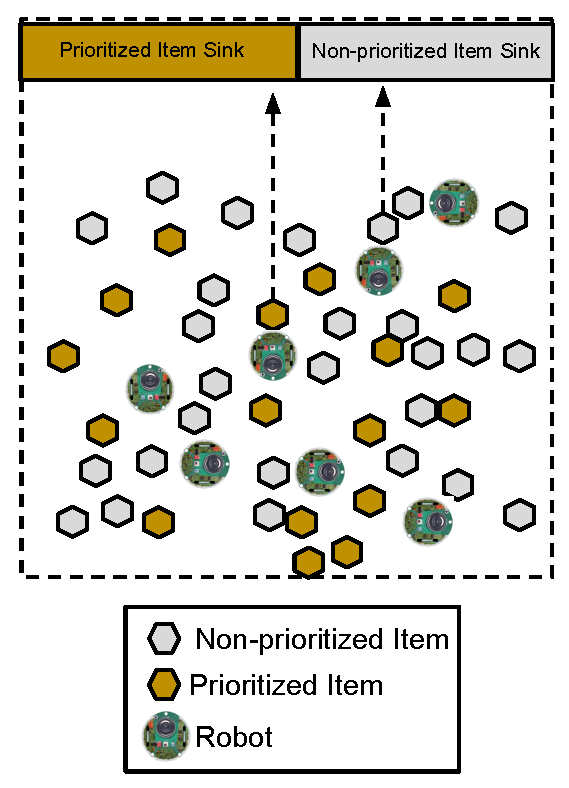
\includegraphics[width=0.65\textwidth]{chapters/chapter2/figures/EpuckGoldMining.pdf}
	\caption{Prioritized Foraging Problem }
	\label{prioritizedforaging}
\end{figure}

As per Winfield's classification described in section \ref{sec:second:taxonomy}, the prioritized foraging problem has a constrained environment, multiple source areas with multiple sinks, multiple object types, object placement is tested in a number of environment types explained in the following sections. There are multiple homogenous robots with limited sensing, relative localisation with near communications and unlimited power. Power is kept as unlimited since the energy preservation of algorithms is to be studied as a performance measure. 

%%%%%%%%%%%%%%%%%%%%%%%%%%%%%%%%%%%%%%%%%%%%%%%%%
%%%%%%%%%%%%%%%%%%%%%%%%%%%%%%%%%%%%%%%%%%%%%%%%%
\section{Summary}
\label{foraging:summary}

%%%%%%%%%%%%%%%%%%%%%%%%%%%%%%%%%%%%%%%%%%%%%%%%%
%%%%%%%%%%%%%%%%%%%%%%%%%%%%%%%%%%%%%%%%%%%%%%%%%
%\bibliographystyle{}
%\bibliography{chapter2}

\chapter{Division of Labour}
\label{chap:divisionoflabour}

Due to the importance of division of labour in this research, a variety of division of labour strategies from social insects should be highlighted, explored and contrasted. This chapter defines division of labour as well as analyses different types of division of labour that occur in social insects. Lastly, division of labour strategies employed by different swarm robotics algorithms are employed. 

\section{Definition}
\label{sec:second:definition}

Oster et al. defines division of labour as a "stable pattern of variation" among individuals within a swarm in terms of the repertoire of tasks that individuals perform where each individual specializes on a subset of the complete repertoire of tasks performed by the swarm and the subset of tasks varies across individuals in the swarm \cite{oster1978caste}.  
More simply, Robinson et al. define division of labour as the adjustment of ratios of workers engaged in different tasks based on external and internal stimuli \cite{robinson1992regulation}.

There are two types of division of labour in social insects: 
\begin{itemize}
	\item Temporal polyethism - The pattern of tasks being performed by a worker correlates to the age of the worker. In nature, the younger workers may perform tasks within the nest while the older workers perform tasks outside of the nest.
	\item Morphological polyethism - A worker with some extreme features in terms of size or shape, will specialize more in particular tasks and the more extreme that feature is, the narrower the repertoire of the of the worker. In nature, for example, larger workers would be more likely to form part of defence of the nest. \cite{beshers2001models}
\end{itemize}

%NEED SOMETHING HERE

%include if we find we need. for now, you're done
%\subsubsection{Task Selection}
%Before addressing the different models of division of labour, it's important to discuss one of the main distringuishing characteristics of division of labour: How does an individual select tasks? Much of the study of division of labour is related to how workers select tasks. The factors contributing to the decision are divided into internal and external factors. Internal factors refer to neurological, hormonal, experience or genetic factors where as the external factors refer to environmental stimuli, worker to worker interaction and communication of the increasing need of workers assigned to a particular task. \cite{beshers2001models}.

%Research around task selection is focused around the following topics: 
%\begin{itemize}
%	\item The rules guiding the decision process in workers
%	\item The process of how information about the environment and social stimuli is gathered
%	\item The internal choice mechanism for making the decisions
%\end{itemize}

\section{Models of Division of Labour from Biology}

Beshers at al \cite{beshers2001models} provide a extensive overview of models of division of labour in insects. Due to the use of insect division of labour addressed by algorithms developed in this thesis, an overview of existing models is provided in the next section.

\subsection{Response Threshold Model}

In the response threshold model, workers have intrinsic thresholds for reacting to task-specific stimuli. The variation in task thresholds among workers in a swarm induces the division of labour \cite{robinson1992regulation}. The response threshold model identifies variation in the worker environment interaction as the primary reason for division of labour

Each task in the repertoire has a related response threshold. The default state of all workers is to have no task assigned. All workers have some threshold for a task and higher stimulus levels result in recruitment of additional workers into a task group. Specialist have the lowest thresholds for a particular task. A negative feedback loop is formed because as the performance of a task by a worker increases, the stimulus level of that task decreases. If a worker with a lower threshold reaches a task then the worker with the higher threshold may never reach that threshold and thus will never perform the task \cite{beshers2001models}.

The simplicity of the response threshold model makes it a popular choice for division of labour in swarm robotics, however it suffers from a number of problems. A predominant problem is that a small intrinsic variation in the performance or responsiveness of a workers' ability to complete task may be amplified into large differences in task repertoire or the frequency of task performance. 

The response threshold model makes the assumption that all workers are equally likely to encounter each task and that stable equilibrium is reached when the number of workers performing a task matches the stimulus level and when individual workers maintain constant task performance probabilities \cite{page1990self}.

\subsection{Integrated Threshold--Information Transfer Model}
\label{integratedthreshold}

Integrated Threshold Information Transfer model can be discerned from it's name. Workers perform a task when the stimulus they encountered equals an internal threshold - the internal threshold will vary according to genetics. The process of discerning a task stimulus is known as information transfer. Information transfer can be perceived randomly in space, directly or via social information transfer  \cite{fewell1999division}. In Integrated Threshold-Information Transfer, both the integrated threshold can be varied as well as the method of transferring information.

Fewell et al  use information transfer models to predict swarm level response patterns to graded changes in stimulus levels for the tasks. The model predicted that normally distributed patterns of task thresholds would induce a graded response - independently of how the individuals received information about the task \cite{fewell1999division}.

%NOT VERY GOOD BUT FUCK IT!

\subsection{Foraging for Work}

Foraging for work is controversial in the fact that it induces division of labour without any explicit worker mechanism but instead a natural result of the environment \cite{beshers2001models}.  
Foraging for Work has two main parts:
\begin{enumerate}
	\item Workers repeat the same task when possible.
	\item Workers actively seek work when they have no task.
\end{enumerate}

%This forms the basic model of foraging and also is used in MY honey bee algorithm.

Foraging for work makes the assumptions that workers are intrinsically identical and thus task performance of workers is dependent on opportunity, rather than intrinsic task preferences. However, it has been shown that in true insect colonies, there is intrinsic variation in each worker's response to the environment as not all workers will respond equally. Another assumption is that tasks are radially spatially localized within the nest. That means the tasks further away are performed by older workers and the younger workers will perform the tasks that are nearer.

Foraging for work shows that temporal polyethism doesn't require age-related difference in the mechanism of task choice and can simply stem from the older workers proximity to the nest which is controversial as it sets the base expectation of what level of task organization might occur within a social group in absence of selection efforts or intrinsic mechanism of worker task performance \cite{franks1994foraging}.

Foraging for work can be seen as a special case of the threshold model where all workers have identical thresholds. The observation of this fact is that with Foraging for Work, temporal polyethism is generated by spatial organization, where as in threshold models polyethism is generated by differences in performance threshold. A disadvantage of threshold models is that lazy workers can be generated by those workers with high thresholds resulting in inactive workers where as according to Foraging for work all workers should either be performing or seeking tasks.

\subsection{Self Reinforcement Models}
\label{selfreinforcement}

Task success is directly proportional of the probability of doing the task again. Self reinforcement models answer the question about whether division of labour is generated as a result of experience \cite{lerman2005review}. If a task was not performed successfully or there was the lack of opportunity then the probability of ever performing that task reduces. The result is that task specialists are created. 

A study performed on foraging specializations by Deneubourg et al shows that self-reinforcement paired with worker age variation are to account for temporal polyethism \cite{deneubourg1987self}. Plowright and Plowright use self-reinforcement to generate elitism \cite{plowright1988elitism} determining that the result was a bimodal frequency of performing tasks where the agents either became specialists or became entirely inactive.

Theraulaz introduces the concept of learning and forgetting \cite{theraulaz1998response}. Learning is when there is a reduction in response threshold when a worker performs a task. And forgetting is an increase in response threshold when a worker doesn't perform a task. All individuals begin with equal thresholds. Evidence from the model indicated that workers adequately adjusted activity levels according to the task they ended up specializing in and exhibited flexibility such that when workers of a specific task are removed the swarm would adapt in order to cater for for missing individuals. 

%  /$$$$$$  /$$$$$$$$ /$$$$$$  /$$$$$$$ 
% /$$__  $$|__  $$__//$$__  $$| $$__  $$
%| $$  \__/   | $$  | $$  \ $$| $$  \ $$
%|  $$$$$$    | $$  | $$  | $$| $$$$$$$/
% \____  $$   | $$  | $$  | $$| $$____/ 
% /$$  \ $$   | $$  | $$  | $$| $$      
%|  $$$$$$/   | $$  |  $$$$$$/| $$      
% \______/    |__/   \______/ |__/      
%NB: ABOVE is what happens in my own things
                                   
\subsection{Network Models of Task Allocation}

Network models of Task allocation, developed in \cite{gordon1992parallel} and extended upon in \cite{pacala1996effects} are a model of simple interactions between workers. It assumes that workers are identical and instead division of labour is induced directly by effective communication of the number of workers required per task between workers. 
 
In this particular network allocation models a worker performs one of four tasks, where for each task they are either active or inactive. This results in each worker having 8 states. Workers having the same states belong to the same task group and all worker interactions are bias towards transferring information with workers that belong to the same task group \cite{gordon1992parallel}. The worker behaviour in each iteration is determined by a linear combination of interactions. The system moves to a balance of active and inactive workers. 

Pascala \cite{pacala1996effects} developed a differential equation to investigate the effects of social group size on task allocation. Information was received directly from the environment, through success or failure of task performance and random encounters with other group members. It was shown that large networks (ie a large number of agents) track environmental changes more efficiently as there is a higher rate of information flow but interaction increases substantially causing interference. Thus as colony size increases, the overhead from interactions becomes faster than the information collection rate from the environment. The solution is to limit the frequency of interaction \cite{pacala1996effects}

The key similarity between network models and foraging for work models is that despite the fact that goals differ, they both share the view that division of labor can be generated by changes in local information encountered by an individual worker. Local information is affected by availability of performance of other tasks, resulting in workers switching between task spaces. Network models are more accurate than the linear model of foraging for work, but network model lacks self organizational properties of foraging for work models.

\subsection{Social Inhibition Models}

The sheer presence of older foraging bees affects behavioural development as the proportion of bees becoming foragers is indirectly related to the number of older bees present in the swarm \citation{huang1992honeybee}. This effect is modelled in the activator-inhibitor model.

Activator-Inhibitor model is driven by 2 hormones:
\begin{itemize}
	\item The activator hormone which is the juvenile hormone that motivates the workers in the hive to become foragers.
	\item The inhibitor hormone which is transferred from the foragers to the younger workers, suppresses the bees development into foragers. If foragers are lost in an accident then more hive workers will mature to foragers due to the decrease of the level of the inhibitor hormone.
\end{itemize}

The mathematical version of the social inhibition model represents the workers physiological state by a single variable $x$ that changes daily in response to the social environment \cite{beshers2001social}. The model defines the trajectories for behavioural development that is intrinsically determined and responsive to social environments. Task performance is correlated with age. Social inhibition provides mechanism of changing worker thresholds as they age which response thresholds fail to do. Social inhibition models allow swarms to flexibly respond to dynamic environments. %pointsless but fuck it!%

\section{Division of Labour in Robot Swarms}

Numerous division of labour strategies have been used in robot swarms. Labella et al. \cite{labella2006division} develop a division of labour strategy for prey retrieval based on Deneubourg's ant self re-enforcement model as discussed in \ref{selfreinforcement}. Experimentation was performed on real robots as well as in simulation. Robots change from search to rest with probability $p$. This probability gets incremented when a robot successfully returned to the nest with an item and decremented when a robot returns to the nest without an item. They classified the foragers into different types based on the final value of $p$ - loafers, foragers and undecided and showed that the values of $p$ tended towards extremes showing that in general, robots tended to become either loafers or foragers, while only a few became undecided. It was shown that a simple self-reinforcement division of labour model can improve the performance of a swarm of robots at a task without the need for communication, however scalability is still a concern as there are negative effects as group size increases. In the author's opinion, this shows that division of labour is not entirely effective since algorithm able to to effectively divide labour would decrease the number of robots performing a specific task if there are too many robots performing the task.

Agassounon et al. design and demonstrate three threshold-based methods for division of labour\cite{agassounon2002efficiency} on clustering a number of small objects in order to dynamically allocate the most appropriate number of robots to the task. The idea is that initially there will be multiple possible sites for clustering, however later in the clustering process, having too many robots competing for a single site will cause interference decreasing the efficiency of the process. The experiment determined that the swarm benefited from threshold division of labour since the algorithms with division of labour performed similarly or better than those with a fixed group size. 

\begin{itemize}
\item The first algorithm, PrFT, does not use explicit communication and assigns fixed response thresholds to the robots.
\item The second algorithm, PrVT, does not use explicit communication and assigns variable response thresholds to each robot. 
\item The final algorithm, PuFT, makes use of explicit peer-to-peer communication between robots to communicate the worker demand but assigns fixed response thresholds to the robots.  Communication occurs when robots are in each other's communication range. The final worker threshold is calculated by averaging the worker threshold's from all robots in the communication range with their own sensed worker threshold. 
The PuFT algorithm is an example of Integrated Threshold -- Information Transfer as described in section \ref{integratedthreshold}.
\end{itemize}

In conclusion, the study determined that after a priori optimization of the fixed thresholds the algorithms performed comparatively similarly. PuFT appeared to perform the best, however the cost of communication was not included in the study. This result can possibly be attributed to the fact that information transfer increased the spread of environmental knowledge and thus the speed at which the division of labour parameters were adapted. Both fixed threshold algorithms suffered badly in environments where they were not optimized for. They pose that an algorithm combining the advantages of threshold variability and information sharing would be worth exploring. 

Liu et al. \cite{liu2007towards} introduce 3 mechanisms for adapting the number of resting robots to foraging robots in a simple foraging problem. The mechanisms consist of variations on how one perceives the worker demand: internal success at task, collective success at task and environmental interference while performing a task - specifically collisions with other agents. The algorithms modify time specific thresholds of how long to wait before going back to work and how long to work for. Four combinations of these factors are evaluated as well as compared to a nai\"ve foraging approach. The efficiency of the swarm is evaluated and compared at different food densities and robot quantities and evaluate energy spend as an efficiency metric rather than number of items foraged over time. %results

To conclude, it appears majority of existing division of labour research is focussed on determining the most efficient number of foragers that should be active at a time. The discussed division of labour strategies have been found to be seemingly beneficial in the problem of regulating the number of robots and despite the seeming simplicity of the problem - to perform a single task or not, the ability to regulate the number of robots is a key requirement of a swarm robotics system as it affects the flexibility, and scalability of a swarm. The ability to adjust the number of resources required to handle a particular problem results in an swarm with the ability to adapt to dynamic environments and thus increasing overall flexibility of the swarm. It also allows the performance to not degrade when more agents are added to the problem since robots will be able to adequately adjust when too many robots have been added and are decreasing productivity and efficiency. 

That said, there is space for addressing other types of division of labour and task allocation problems besides that of optimal number of active robots as many systems require division of labour between multiple active tasks. There is also a lack of implementation of other types of division of labour models such as the network based models which may be worth exploring.

Lastly, despite the general attempt to test scalability, the maximum swarm size is usually 10 or less. It is in the author's opinion that it would be beneficial to attempt this study on a larger scale problem with larger swarm sizes to truly see the benefit in the division of labour strategy to regulate the number of foraging robots. 

\section{Summary}
\label{sec:second:summary}
Division of labour is the adjustment of ratios of workers engaged in different tasks based on external and internal stimuli. Division of labour is used in social insect societies such as bees and ants and multiple models for division of labour have been explored by biologists. Extensive research has been performed about response threshold models, internal threshold information transfer, foraging for work and self-reinforcement models. The different models are explained and compared. Despite the large number of models, little verification of these models have been performed in real or simulate environments. 

Lastly, the use of division of labour in swarm robotics is explored. Most of the reviewed research was focused around the problem of using division of labour to regulate the number of active robots where a robot has two division of labour states - either actively performing the task or resting. The techniques used in swarm robotics employ a variety of division of labour models. The author notes that the reviewed research did not adequately address the scalability of the techniques and discussed how more complex version of division of labour problems still need to be addressed.